\documentclass[a4paper,12pt,twoside]{article}
\usepackage{preamble}
\usepackage{amsmath, amssymb, amscd, amsthm, amsfonts}
\usepackage[titlepage,fancysections,pagenumber]{polytechnique}

\title{INF567 Project}
\subtitle{Zero-Forcing Beamforming for Visible Light Communication Systems}
\author{Gabriel Pereira de Carvalho}

\date{\today}

\begin{document}
	
	\maketitle
	
	\tableofcontents
	
	\newpage
	
	\section{Introduction}
	
	Today, the processing power of edge devices (embedded systems on the frontier between computer networks and the physical world) allows them to perform more and more tasks independently. The networks connecting these devices (Internet of Things or IoT) has experienced tremendous growth.
	
	However, the RF technologies used for these networks (Wi-Fi, 4G or 5G) are experiencing more and more congestion due to the limited bandwidth available to all devices sharing the medium. In the literature, this problem is called \textbf{Spectrum crunch}.
	
	The visible light spectrum used by Visible Light Communication(VLC) technologies is approximately 10000 times larger than the entire radio frequency spectrum. This means less congestion, less interference and speeds higher than what is achievable with radio frequencies. Lab tests have achieved data rates of up to 224 gigabits per second. And since light cannot penetrate walls, it's much harder for potential hackers or unauthorized individuals to access a VLC network.
	
	The messages are transmitted using rapid fluctuations in LED light intensity (so fast they are invisible to the human eye). This means that LED lamps in a VLC network can provide light and simultaneously transmit data.
	
	The goal of this project is to explore the \textbf{zero-forcing beamforming} technique proposed in \cite{Oxford2021} for Physical Layer Security(PLS) to prevent both active and passive eavesdropping on VLC systems and attempt to replicate their results.
	
	The literature review performed on \cite{Edinburgh2020} was the basis for the bibliography study performed on this project. It is important to highlight that VLC systems are not intended to replace RF technologies. VLC systems are more efficient in indoor environments and are complementary to RF technologies.
	
	\subsection{Modelisation of Indoor VLC system}
	
	The modulation/demodulation scheme analysed in \cite{Oxford2021} and considered for this project is IM/DD where \textbf{IM} (intensity modulation) refers to the method of encoding information by varying the intensity of the light source, which is then detected by a receiver. And \textbf{DD} (direct detection) refers to the detection of the transmitted signal by directly measuring the intensity of the received light, typically using a photodiode, without needing to decode phase or frequency information.
	
	We consider an IM/DD MIMO VLC system with:
	\begin{itemize}
		\item multiple Access Points(APs);
		\item a single Authorized User(AU);
		\item multiple Active Eavesdropping Devices(AEDs);
		\item and multiple Passive Eavesdropping Devices (PEDs).
	\end{itemize}
	
	\begin{figure}[h!]
		\centering
		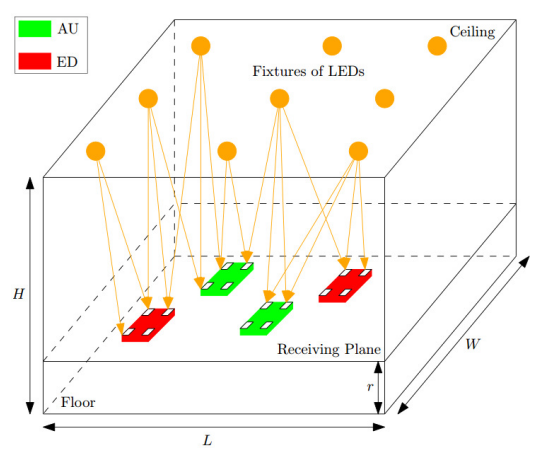
\includegraphics[scale=0.5]{../modelisation.PNG}
		\caption{Generalized model for MIMO VLC system \cite{Edinburgh2020}}
	\end{figure}
	
	As in \cite{Edinburgh2020}, we consider a room os size $L \times W \times H$. The room is equipped with $N$ APs that are located at its ceiling. The APs act as single transmitters, sending simultaneously the confidential message signal $s(t)$ to the AU in the presence of $P$ known AEDs $\{ AE_1, AE_2, ..., AE_P \}$ and $Q$ unknown randomly distributed PEDs $\{ PE_1, PE_2, ..., PE_Q \}$. We use the index $k \in \{AU, AE_p, PE_q\}$ to refer to a generic device.
	
	\subsection{Zero-Forcing Beamforming}
	
	Ideally, we want to maximize the SNR at the AU, and make it zero at every eavesdropping device. We can impose this constraint at the AEDs, whose position is known but it is more complicated to consider the PEDs whose position is unknown. We will discuss how to treat PEDs later in the report.
	
	Our goal is to determine the beamforming vector $w = [w_1,w_2,...,w_N]^T \in \mathbb{R}^N$ where $w_i$ is a weight for the signal from the $i$-th transmitter satisfying $\forall i \in \{1,2,...,N\}$:
	
	\begin{align}
		\begin{cases}
			w_i \in \mathbb{R} \\
			|w_i| \leq 1
		\end{cases}
	\end{align}
	
	Each AP will transmit a modulated signal $x_i(t)$. The LEDs are modelled as \textbf{Lambertian light sources}, which means that the observed luminous intensity is directly proportional to the cosine of the angle  $\psi_{i,k}$ between the observer's line of sight(\textbf{LoS}) and the surface normal
	\begin{equation}
		I = I_0 \cos( \psi_{i,k})
	\end{equation}
	this law is known as Lambert's emission law. We also define the angle of irradiance $\phi_{i,k}$ between the LoS and the surface normal at the AP.
	
	\begin{figure}[h!]
		\centering
		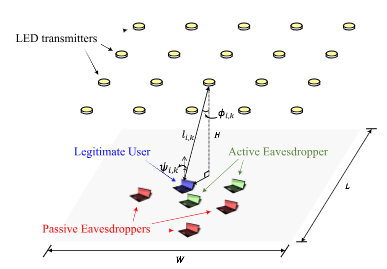
\includegraphics[scale=0.8]{../geometry.PNG}
		\caption{Geometrical parameters in the generalized VLC model \cite{Oxford2021}}
	\end{figure}
	
	For each device, we also introduce the channel gain vector $h_k = [h_{1,k}, h_{2,k}, ... , h_{N,k}]^T \in \mathbb{R}^N$ which models the effect of the channel on the signal during propagation. Reflections are ignored and only the direct path from source to receiver (LoS path) is considered. In \cite{Oxford2021} many physical constants are introduced, we will simply use $\mathbb{C}$ to simplify the notation. We have
	\begin{align}
		h_{i,k} =
		\begin{cases}
			\mathbb{C}\frac{\cos(\phi_{i,k})}{\sin(\Psi)^2}\cos(\psi_{i,k}) \qquad &\text{for $|\psi_{i,k}| < \Psi$} \\
			0 \qquad &\text{for $|\psi_{i,k}| > \Psi$}
		\end{cases} 
	\end{align}
	where $\Psi$ denote the photodiode's field of view. As in \cite{Oxford2021}, we will take $\Psi = 90^\circ \implies \sin(\Psi)^2 = 1$.
	
	The modulated signal $x_i(t)$ is related to the message $s(t)$ by the relation
	\begin{equation}
		x_i(t) = \alpha I_{DC} s(t)
	\end{equation}
	where $\alpha \in [0, 1]$ is the modulation index and $I_{DC} \in \mathbb{R}_+$ is the current used by the AP LED for illumination. 
	
	By the superposition principle, the signal $y_k$ received at device $k$ is the sum of the signals received from each AP which gives
	\begin{equation}
		y_k(t) = \alpha I_DC (h_k \cdot w) s(t) + n_k(t)
	\end{equation}
	where $n_k(t)$ represents white Gaussian noise.
	
	\section{Beamforming with one AED}
	
	The traditional zero-forcing beamformer for a single AED $AE_1$, where the PEDs are ignored, can be obtained by projecting the AU's channel onto the null space of the AED (making the SNR at the AED equal to zero).
	
	\section{Beamforming with multiple AEDs}
	
	
	\section{Beamforming with multiple AEDs and PEDs}
	
	
	\newpage 

	\begin{thebibliography}{9}
		\bibitem{Edinburgh2020} Mohamed Amine Arfaoui, Mohammad Dehghani Soltani, Iman Tavakkolnia, Ali Ghrayeb, Majid Safari, Chadi M. Assi, Harald Haas (2020). \textbf{Physical Layer Security for Visible Light
		Communication Systems: A Survey}. IEEE Communications Surveys and Tutorials.
		
		\bibitem{Oxford2021}
		Sunghwan Cho, Gaojie Chen, Justin P. Coon (2021). \textbf{Zero-Forcing Beamforming for Active and Passive Eavesdropper Mitigation in Visible Light Communication Systems}. IEEE Transactions on Wireless Communications.
	\end{thebibliography}
	
\end{document}